\documentclass[../main.tex]{subfiles}

\begin{document}

\section{Overview}

This chapter presents the goals and development of the LeafAI web application, an interactive user-facing web interface which integrates with the LeafAI API described in Chapter \ref{chap:query_generation}. As development of the web application is in progress, we leave evaluation of this to future work. Section 8.2 describes related work. Section 8.3 describes methods. Section 8.4 discusses future work, including user testing, and Section 8.5 concludes this chapter. 

\section{Related Work}

Experimental systems enabling the querying of databases using natural language interfaces have been in development since the 1960s. Using relatively simple rule-based parsing systems, Woods \cite{woods1973progress} created a system for asking natural language questions of a moon rock database, while Epstein and Walker \cite{epstein1978natural} similarly designed a natural language interface for a melanoma database. Decades later, Katz \textit{et al} created START \cite{katz1999integrating}, a system capable of basic question-answering using data extracted and parsed from the internet. In the biomedical informatics domain, Cao \textit{et al} developed AskHERMES \cite{cao2011askhermes}, question-answering software capable of answering medical questions related to drugs, contraindications, and so on, using support vector machines (SVMs) and an internal knowledge base derived from the UMLS.

Cohort discovery systems using natural language are in many ways a subset of systems for question-answering which answer only one (unstated) question, "How many patients meet these criteria?". As discussed, in the biomedical informatics and clinical trials domain, the most well-known and cited system for matching patients to clinical trials using free-text eligibility criteria is Criteria2Query \cite{yuan2019criteria2query, fang2022combining}. Criteria2Query offers a web-based simple and friendly user interface for inputting free-text eligibility criteria and enables users to correct erroneously normalized named entities.

\section{Methods}

The web application forms one component of the LeafAI application, which is a 3-tier architecture similar to Leaf \cite{dobbins2019leaf}: a back-end with clinical and application databases, and server hosting an API (Chapter \ref{chap:query_generation}), and a user-facing web application. The web application features a chat-like design.

A chat-like interface for cohort discovery is both novel and a logical design choice given the natural language interface of LeafAI used for query generation. An example of LeafAI's user interface is shown in Figure \ref{fig_leafai_demo}. As can be seen, we assume that the order of user-provided criteria is intentional and important, and leverage that assumption to both structure queries incrementally to report results line by line, with each reported result (e.g., "421 are aged between 18 and 65") effectively a subset of the preceding result.

\begin{figure}[h!]
  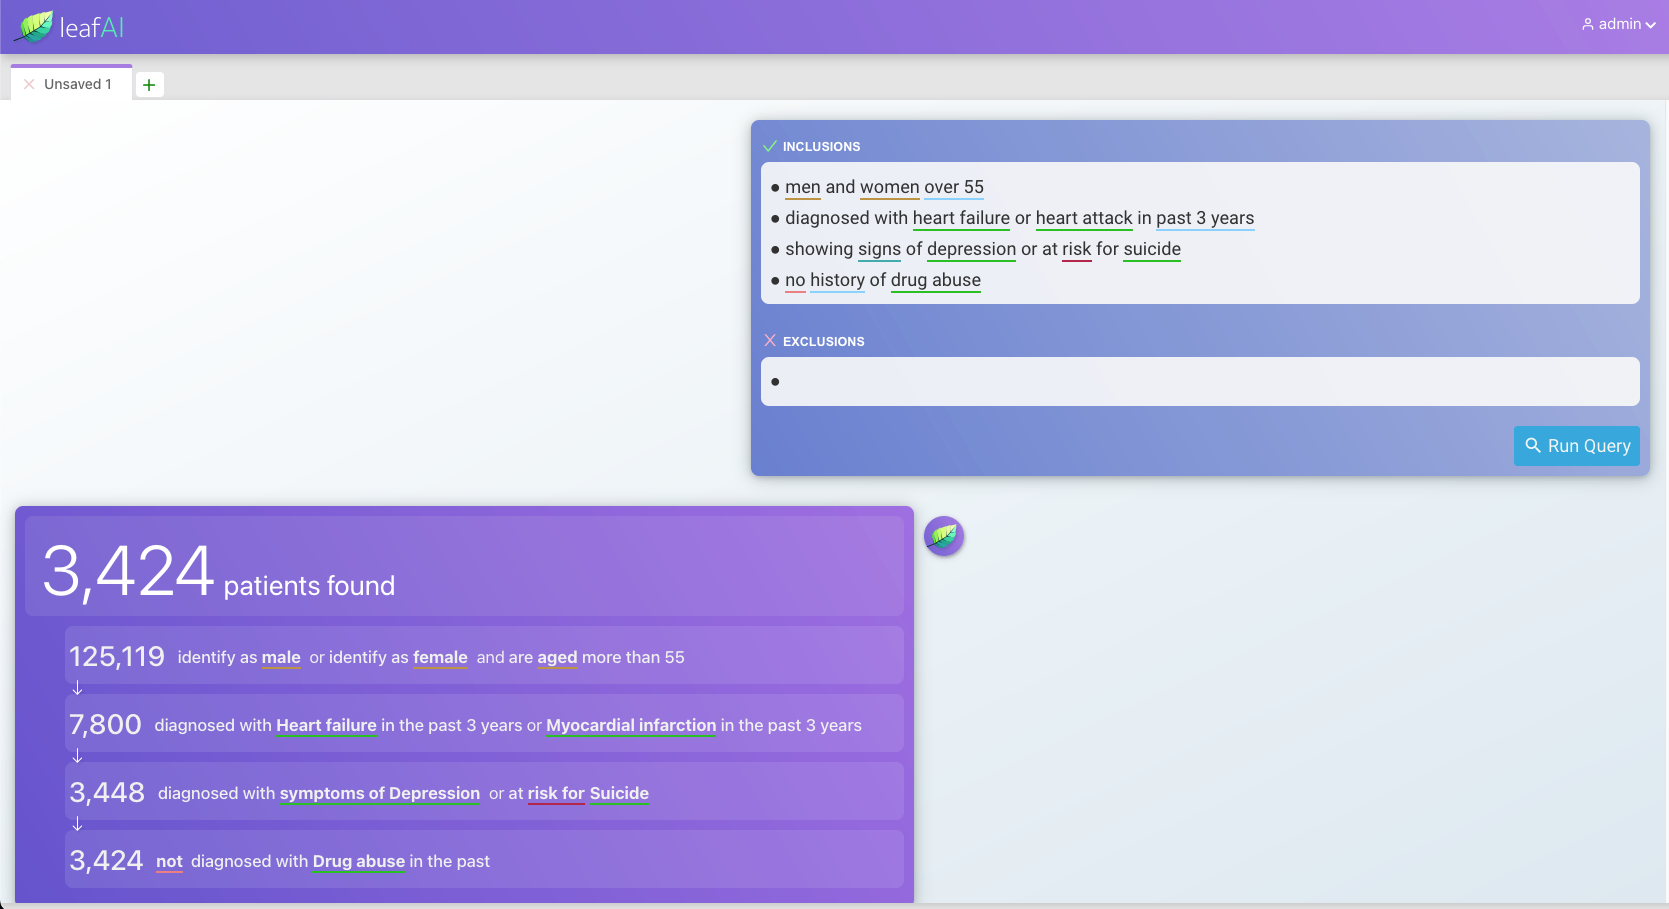
\includegraphics[scale=0.28]{Figures/8_web_application/leafai_demo.png}  
  \caption{The web application user interface. User-entered criteria are shown in the above right, while system responses are shown in the lower left. User criteria are displayed and executed in order, with each count of patients representing a subset of the preceding count.}
\label{fig_leafai_demo}
\end{figure}

The web application responds to user input in a visual form that is chat-\textit{like}, rather than the result of a general programmatic conversation agent. While the user interface and query generation methods lay a potential foundation for general-purpose question-answering more akin to a conversation agent, we limit our scope to cohort discovery. The user interface was designed with the following goals:

\begin{enumerate}
    \item \textbf{Accessible history}. Users will be able to immediately scroll to view previous findings.
    \item \textbf{Rapid feedback and explainability}. The application performs NER and normalization as users type. This allows users to preemptively detect concepts and queries which may return unexpected results. The application also returns incremental query results in real-time, providing immediate feedback so users may avoid waiting until all query results are complete.
    \item \textbf{Direct editing of responses enabling iteration}. As the application returns results of patients found, the eligibility criteria used in a query will be directly edit-able, saving users' time and facilitating quick iteration to find intended patients.
\end{enumerate}

\noindent We next describe each goal in detail.

\subsection{Accessible History} 

Cohort discovery is a form of data exploration. As Derthick and Roth write, "...the data exploration process is not characterized by monotonic progress towards a goal, but rather involves much backtracking and opportunistic goal revision" \cite{derthick2001enhancing}. Put another way, user goals and perceptions may change over the course of exploration. With ubiquitous vertical scrolling - where more recent actions and utterances are inserted downward while history is preserved upward - chat-like user interfaces facilitate user understanding of past utterances and actions. Persisted, easily viewable history of user utterances and actions enable what Gergle \textit{et al} call "conversational grounding" \cite{gergle2004persistence}, that is, accessible data to guide users to previously acquired findings and information. This history of previous actions can improve the pace of discovery and alleviate the need for users to (often imperfectly) attempt to recall their earlier findings and paths taken \cite{hill1994history, gergle2004persistence}.

\subsection{Rapid Feedback and explainability}

Users' sense of system latency and responsiveness can significantly affect their satisfaction in using a tool \cite{li2019effects, arapakis2014impact, shneiderman1984response}. Faster \textit{preemptive} system responses (i.e., informing users' of a possible consequence before they complete an action) can also both save users' time and reduce loads placed upon systems by preventing unnecessary actions \cite{lempel2003predictive, diaz2016search}. The web application employs two general strategies for providing rapid feedback to users, one before queries are executed, and the second while results are being reported during query execution.

Consider a hypothetical case where a user begins to type a criteria but misspells "Diabetes Mellitus". Given no notification of the error, the user may take seconds or even minutes of additional typing while adding new criteria without realizing the initial spelling mistake. After the user awaits LeafAI's response, she finds that the query found no patients and is frustrated and confused at the counter-intuitive result, only to finally notice the misspelling, having wasted several minutes. The application avoids this scenario by preemptively performing NER and normalization while users are typing. Examples of this are shown in Figure \ref{fig_leafai_mouse_hover}. Named entities found within user criteria are underlined and interactive, enabling users to better estimate whether their queries will succeed or not.

\begin{figure}[H]
  \centering
  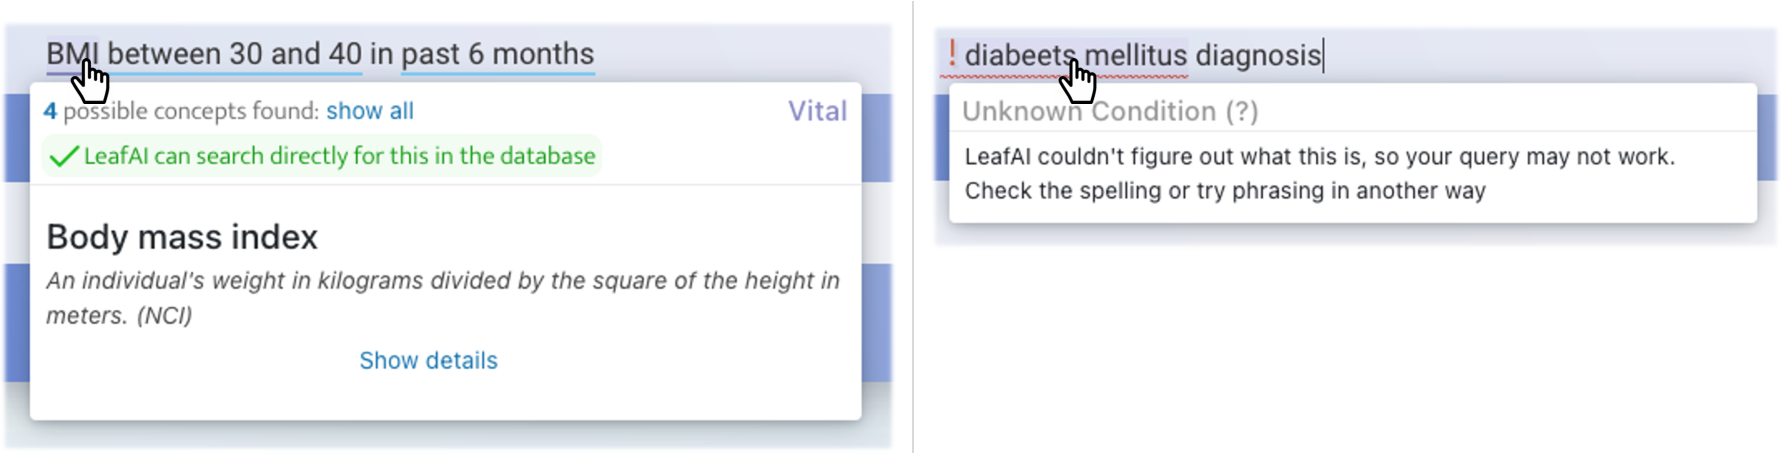
\includegraphics[scale=0.55]{Figures/8_web_application/leafai_normalization.pdf}  
  \caption{Normalized named entities identified in user input before query execution. On the left, the system correctly identified "BMI". On the right, "Diabetes Mellitus" is misspelled, and the user is notified.}
\label{fig_leafai_mouse_hover}
\end{figure}

Second, as LeafAI generates incremental queries and returns results line by line asynchronously, the user interface shows results as they are reported using a streaming interface. As a result, users do not need to wait until all queries are complete to obtain visual feedback as to query results (as in tools such as Leaf and i2b2). An example of this is shown in Figure \ref{fig_leafai_query_progress}.

Taken together, these features for rapid feedback and transparency also enable \textit{explainability} of system actions. Rather than simply returning a final count of patients meeting criteria, The user interface provides information both before and during query execution of how the system interpreted user intent and how it has executed a query (e.g. what concepts it found or did not, misinterpreted, etc.). System responses are generated using templated English expressions mapped to logical form types using normalized UMLS concept names. By avoiding being a "black box", the user interface is designed to gain user trust and understanding of how the system operates.

\begin{figure}[H]
  \centering
  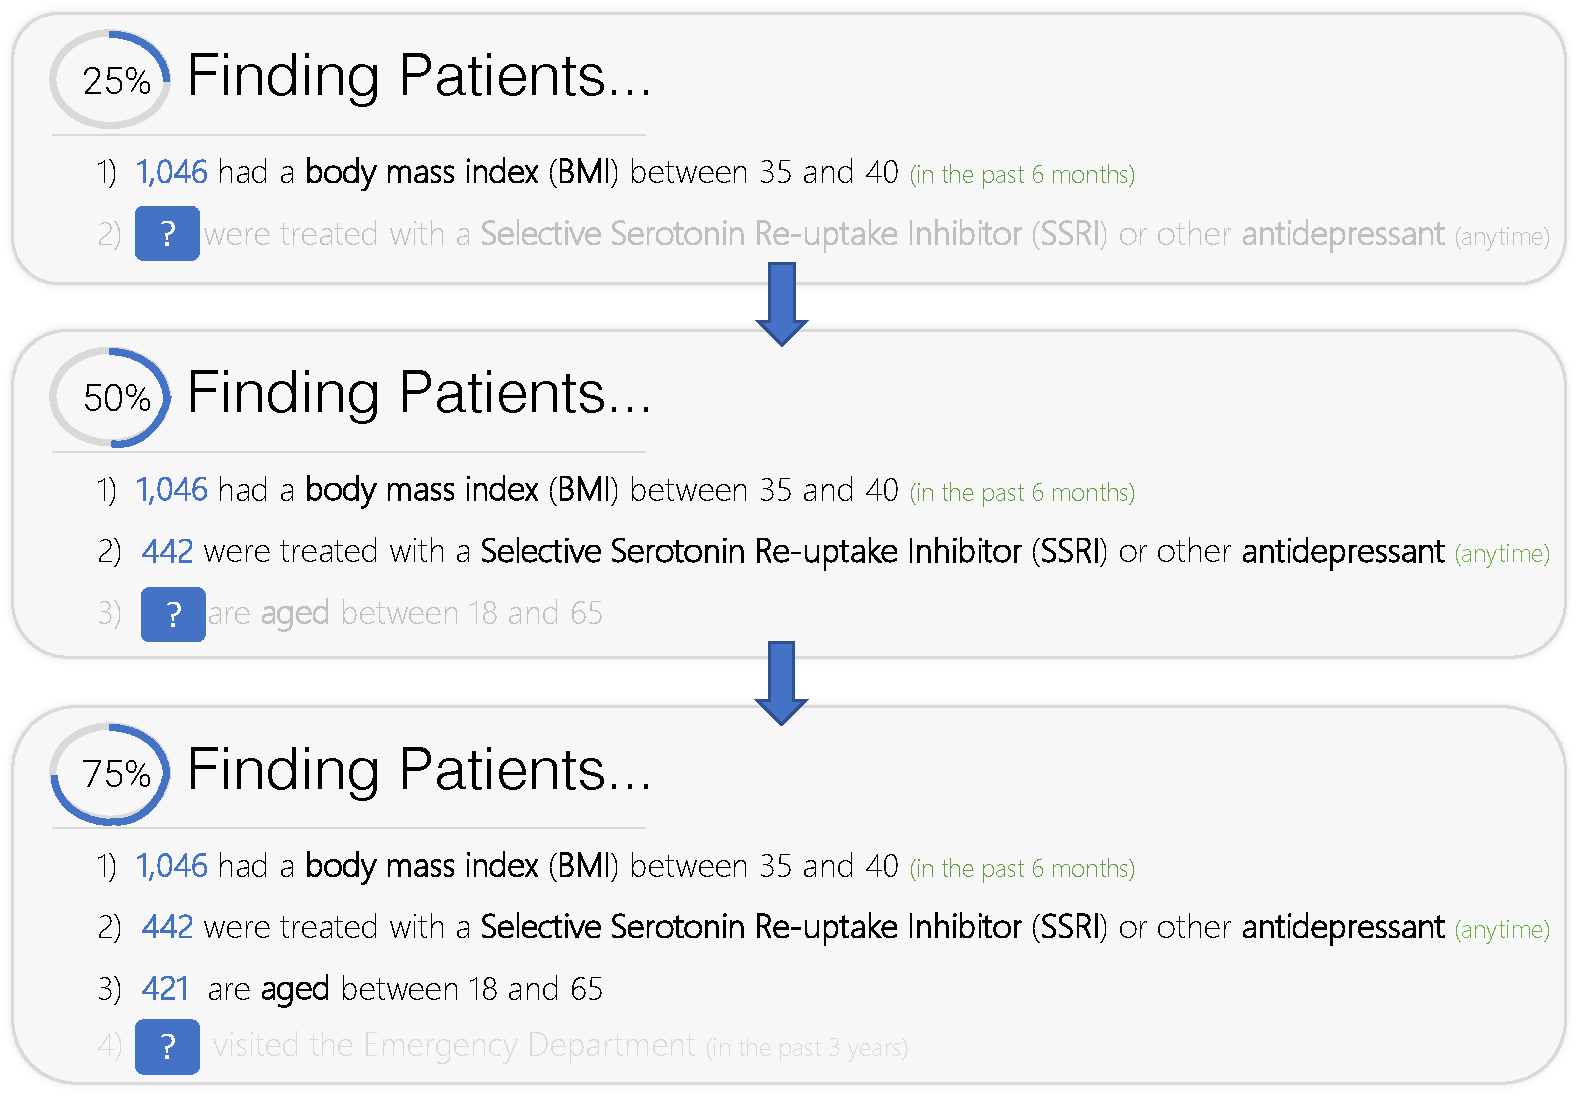
\includegraphics[scale=0.65]{Figures/8_web_application/leafai_query_progress.pdf}  
  \caption{A time-lapse representation asynchronously reporting of incremental query results, from top to bottom. This is performed using two streaming interfaces, one from the clinical database to the API, and a second from the API to the web application.}
\label{fig_leafai_query_progress}
\end{figure}

\subsection{Direct editing of responses enabling iteration}

Data exploration is iterative: users explore, try, and learn over the course of multiple attempts. As discussed, faster, meaningful results also directly affect user satisfaction. To this end, the web application enables users to immediately and directly edit the returned system responses. This workflow is depicted in Figure \ref{fig_leafai_feedback_loop}. 

\begin{figure}[h!]
  \centering
  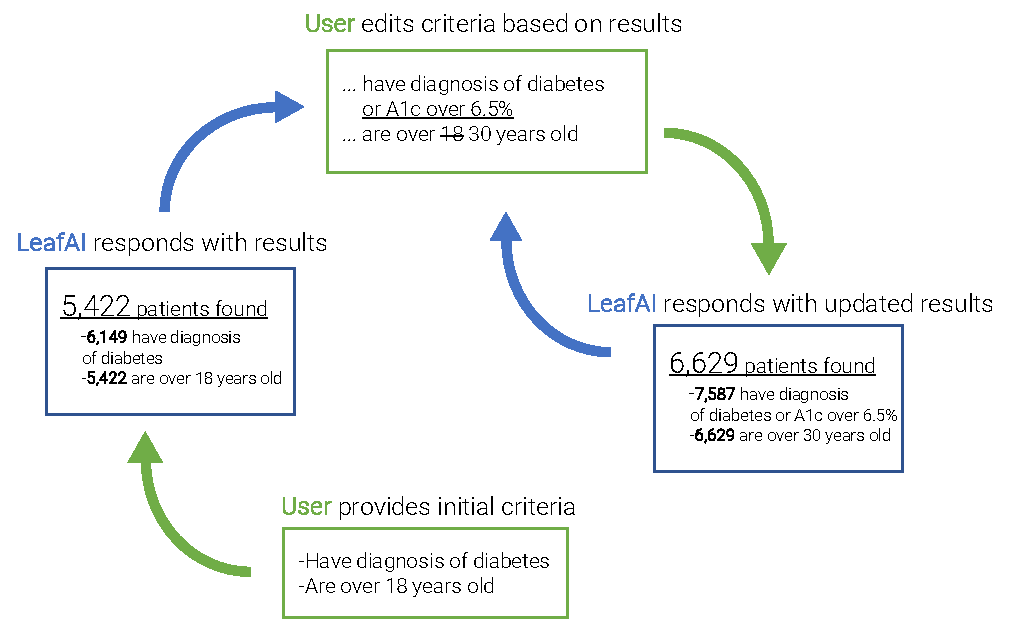
\includegraphics[scale=1]{Figures/8_web_application/leafai_feedback_loop.pdf}  
  \caption{An iterative workflow using an example case for adults with Diabetes Mellitus. Users are able to directly edit results and re-execute their queries while preserving query history, saving user time and preserving previous user actions and findings.}
\label{fig_leafai_feedback_loop}
\end{figure}

For example, after seeing that LeafAI found less patients than expected, a user may realize that she should slightly alter her original query to expand her search. Rather than needing to copy and paste her earlier criteria, instead she is able to simply click and modify the earlier results.

Additionally, as discussed, the LeafAI query engine is capable of reasoning upon non-specific criteria. In certain cases, however, the system's findings may be incomplete, incorrect, or undesired for various reasons. Rather than forcing users to accept imperfect reasoning, however, the user interface allows users to directly enable or disable reasoned concepts. An example of this is shown in Figure \ref{fig_leafai_edit_concepts}. In addition to reasoned concepts, the interface enables users to enable and disable named entities from system responses and immediately re-execute queries with a single click, shown in Figure \ref{fig_leafai_edit_entities}. This allows for fast iteration and saves user time, obviating the need to alter the original inputs.

\begin{figure}[h!]
  \centering
  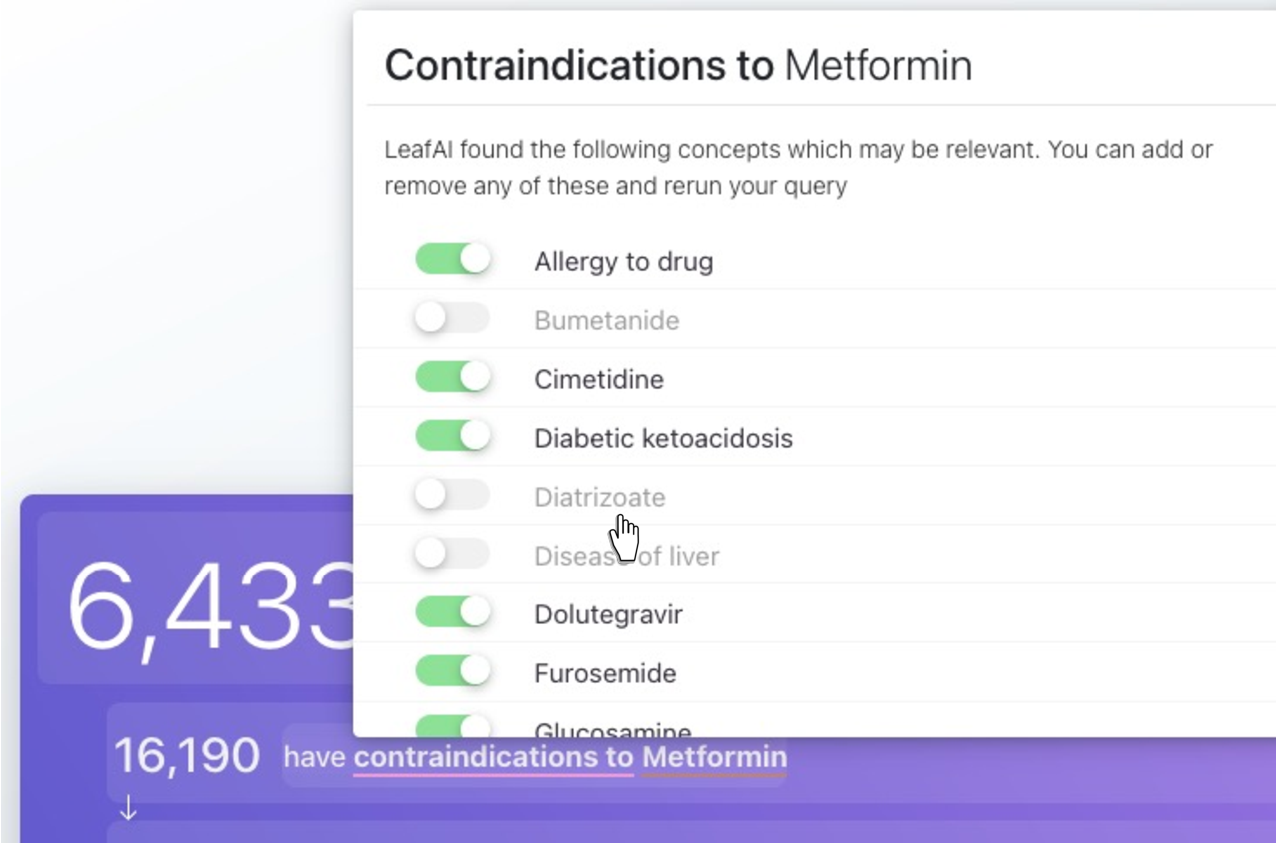
\includegraphics[scale=0.68]{Figures/8_web_application/leafai_edit_concepts.pdf}  
  \caption{An example of a user editing concepts discovered using LeafAI's reasoning system. Users are able to enable or disable reasoned concepts.}
\label{fig_leafai_edit_concepts}
\end{figure}

\begin{figure}[h!]
  \centering
  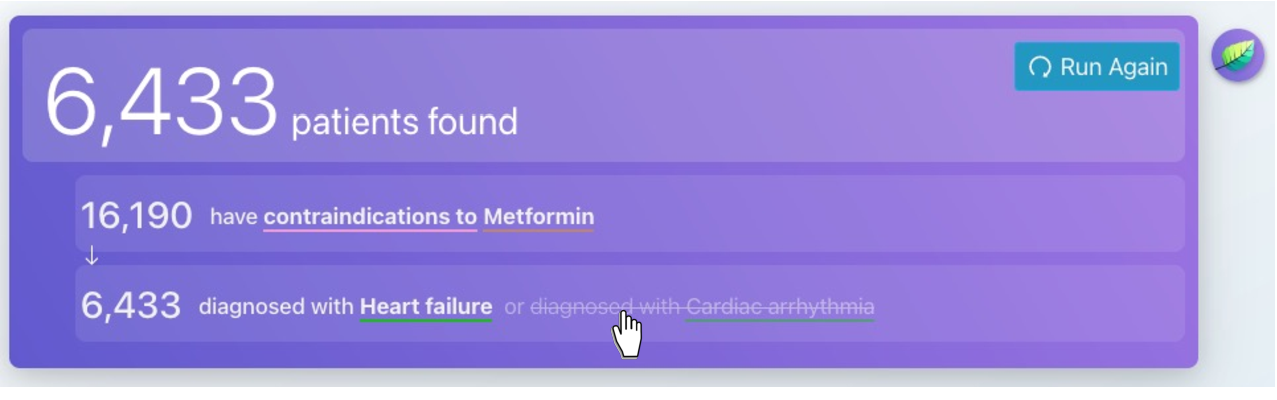
\includegraphics[scale=0.68]{Figures/8_web_application/leafai_edit_entities.pdf}  
  \caption{An example of a user disabling a named entity from a system response. Named entities can be enabled and disabled by clicking directly on them. Disabled entities are shown with gray colored text and struck through by a line. Upon re-execution, logic for disabled entities is removed from the generated query.}
\label{fig_leafai_edit_entities}
\end{figure}

The system's reasoning can thus be described as an optional means of helpfully saving users' time, which can be accepted, edited, or discarded as needed.

\subsection{Model Inference Speed}

LeafAI's modules for NER, logical form transformation, lab normalization and so on use large Transformer-based neural models \cite{vaswani2017attention} with millions of parameters. Using these models as-is for inference can be slow, particularly when performed using CPUs rather than more costly but often far faster GPUs (Graphics Processing Units). Delays in inference time in turn can result in poor system latency, affecting user satisfaction. We further assume that institutions or individuals deploying LeafAI may not necessarily have access to GPUs. To improve inference speed on CPUs, models are quantized, a process for converting 32-bit floating point values within model weights and biases to 8-bit integers. Quantization has been shown to dramatically reduce model storage size and memory usage and improve inference speed while typically showing limited decreases in performance \cite{hubara2017quantized}. 

\section{Future Work}

In future work we will employ a usability and user satisfaction and acceptability study. We hypothesize that the innovative design of the web application user interface will represent a meaningful advance in user interface design for cohort discovery. Future versions of the application may allow for general question-answering, data visualization, and data analysis as well.

\section{Conclusion}

This chapter described the ongoing development of the LeafAI web application, which incorporates a number of innovative user-facing features such as streaming interface updates during query execution, real-time named entity recognition and normalization, as well as mixed-modal interaction allowing users to manipulate system responses and re-execute generated queries. In future work we will evaluate the web application in a usability and user satisfaction and acceptability study.

\end{document}